As early as 2001, researchers have proposed the use of a novel, hybrid engine
design for use in supersonic and hypersonic flight \cite{Macheret2001}. In some
ways similar to an earlier program \cite{Gurijanov1996}, it suggested that
magnetohydrodynamic (\acs{mhd}) accelerators were an enabling technology for
hypersonic transport. Briefly, a \acs{mhd} accelerator could be used to
simultaneously produce energy and slow the inlet airflow. This would allow the
use of a conventional turbojet engine at speeds well above its normal
operational range.

However, \acs{mhd} accelerators require an ionized fluid flow. Even at the high
altitudes associated with hypersonic flight, this is not easy to achieve.
Originally, Macheret suggested the use of electron beams, carefully tuned to
coincide with the peak in the ionization cross section in air. However, the use
of electron beams in the ionization of high pressure gases is accompanied by a
large number of technical issues, similar to those of some excimer lasers.
Therefore, in 2002, Macheret et al.\ proposed the use of a \acs{rpnd} to produce
an ``electron beam'' in situ \cite{Macheret2002} akin to the beams observed in
certain \acs{fiw} studies.

The use of a \acs{rpnd} is accompanied by a reduced ionization efficiency in
comparison to an electron beam. However, it reduces the some of the
implementation challenges and Macheret argued that it offered a more efficient
and stable option than breakdown with DC electric fields. Though the densities
of \acs{fiw}s in several air-related chemistries have been measured on several
occassions \cite{Anikin1998, Aleksandrov2007, Aleksandrov2008,
Starikovskaia2006}, similar studies do not appear to exist for \acs{rpnd}s in
air. Therefore, there is a need for electron density measurements to confirm
that \acs{rpnd}s are adequate for the \acs{mhd} accelerator requirements and to
quantify their ionization efficiency.

In addition, previous studies of \acs{fiw}s in air have observed fast gas
heating of molecular systems \cite{Popov2011}. Up to 40\% of the input energy
can be converted into translational energy through dissociation of oxygen and
quenching or electronically excited nitrogen states. As the \acs{rpnd} physics
are very similar to that of the \acs{fiw}, there is the possibility that it may
also cause fast gas heating. In combustion, this can play an important role in
the chemistry, flame holding, and ignition delay. More generally, gas heating
can impact material processing and ionization efficiency. As such, it is
important to develop reliable temperature diagnostics for \acs{rpnd}s in
molecular gases.

This appendix records the development of two diagnostics for an air \acs{rpnd}
at \acs{nasa} Glenn Research Center (\acs{grc}). Measurement of the electron
density was accomplished using millimeter-wave interferometry. Plasma
interferometry measures changes in the phase and amplitude of an electromagnetic
wave which has passed through the plasma \cite{Lieberman2005}. The phase shift
is proportional to the density of electrons while the change in amplitude is
related to the electron-neutral collision frequency. As with other wave-based
techniques, the density resulting from this approach is line integrated. The
translational temperature of the system was measured via

Translational temperatures were measured by analysis of the rotational spectra
associate with the second positive system of nitrogen. Rotational spectra result
from changes in the rotational quanta of a molecule. As the energy spacing of
the rotational levels is generally quite small (often on the order of $10^{-4}$
eV), inter-molecular collisions can easily redistribute them
\cite{Herzberg1950}. Provided enough collisions, the distribution of rotational
states should reflect the distribution of translational energy for the
molecules.

\section{Discharge Apparatus}

Experiments were conducted in a cylindrical vacuum chamber, reproduced in
figure~\ref{fig:nasachamber},
\begin{figure}
  \centering
  \setlength\fboxsep{0pt}
  \setlength\fboxrule{1.0pt}
  \fbox{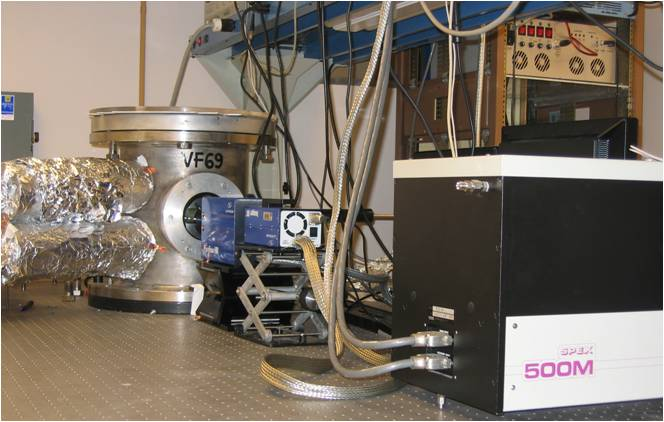
\includegraphics{./chapters/nasa/figures/VF-69.jpg}}
  \caption{Vacuum chamber used in \acs{rpnd} experiments at the \acs{nasa}
    \acs{grc} along with an \acs{iccd} used for fast imaging.}
  \label{fig:nasachamber}
\end{figure}
with a volume of approximately 30 L. The chamber was evacuated by a Varian
TriScroll 300, scroll pump and the pressure was monitored by a capacitance
manometer. Before each experiment the chamber pressure was reduced to below 100
mTorr, after which the chamber was sealed from the pump by a bellows valve. The
chamber was then back-filled with ambient air until the pressure reached 20.0
Torr.

The discharge was sustained between two parallel cylindrical electrodes, 2.5 cm
in diameter and 0.625 cm in length. In the interferometry experiment, the
electrodes were mounted in a silicone-based dielectric epoxy, cast such that it
was flush with the faces of the electrodes. Optical emission experiments
eliminated the dielectric epoxy in favor of a machinable ceramic and slightly
different geometry, seen in figure~\ref{fig:electrodes}.
\begin{figure}
  \centering
  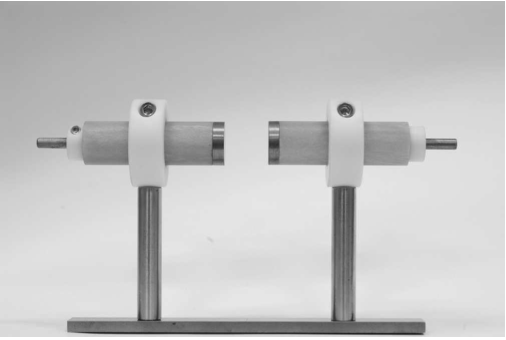
\includegraphics{./chapters/nasa/figures/electrodes.pdf}
  \caption{The electrodes used in the \acs{rpnd} at \acs{nasa} \acs{grc}. The
    electrodes are made of copper with a ceramic sheath made of Mykroy.}
  \label{fig:electrodes}
\end{figure}
This choice was made as a result of damage observed to the epoxy molds. Plasma
breakdown appeared to be occurring at the interface of the mold and the
electrodes. The use of the Mykroy fitting allowed longer duration operation
necessary for the optical emissions measurements.

The power supply was built by FID (model FPG 60-100-MC4-S5) and supplied voltage
pulses of up to 60 kV at repetition rates from 6-100 kHz with pulsewidths of 5
ns. Unless otherwise stated, all measurements were made with the power supply
operating at 20 kHz using a Wavetek FG3C as the master clock.

Maintenance of the electrodes and other components of the discharge apparatus
required that the chamber volume regularly be brought up to atmospheric
pressure. When the discharge was initiated after the chamber was returned to the
20.0 Torr operating pressure, a pressure transient was observed. This transient
caused the chamber pressure to rise by about 2.0 Torr after several minutes of
operation, after which the pressure would remain relatively stable. This was
believed to be caused by the outgassing of the discharge apparatus surfaces.
Throughout operation, the pressure would continue to increase at a greatly
reduced rate, on the order of several tenths of a Torr per minute.

\section{Millimeter-Wave Interferometry}

Traditionally, plasma interferometry has been conducted with microwaves, as the
electron densities in processing plasmas cause readily observable phase shifts
at these wavelengths. However, results from similar \acs{rpnd}s
\cite{Starikovskaia2001} suggested that the electron densities could approach
$10^{13}$ cm$^{-3}$. Such densities exceed the cutoff wavelength of microwave
interferometers \cite{Lieberman2005}. As a result, it was necessary to use
millimeter-wave (\acs{mmw}) interferometry which uses much higher frequencies in
order to avoid this issue.

\subsection{Theory}

The theory underlying interferometry can be found in many plasma diagnostic
textbooks, however the majority of the treatments only concern plasmas in which
there are no neutral particles. In contrast, the work of Akhtar et al.
\cite{Akhtar2003} introduces a frictional force to the derivation which accounts
for the effects of neutral particles. Following this approach, the theory below
provides the necessary set of equations in order to determine the electron
density and collision frequency provided measurements of the \acs{mmw} phase
shift and change in amplitude.

The derivation begins with the motion of electron in an oscillating
electromagnetic field. The position of a charged particle in such a field can be
found from the non-relativistic Lorentz equation,
  \begin{equation}
    \bm{F} = q\left( \bm{E} + \bm{v} \times \bm{B} \right),
    \label{eqn:lorentz}
  \end{equation}
where $\bm{F}$ is the force on the particle, $q$ is its charge, $\bm{E}$ is the
electric field, $\bm{v}$ is the particle's velocity, and $\bm{B}$ is the
magnetic field. In the case of a weak electromagnetic field (such as in
interferometry) the magnetic field component can be assumed to be zero. Without
loss of generality, the equation may be reduced to a single dimension.
Afterward, the drag force which accounts for the neutral particle collisions can
be introduced. The acceleration of the electron can then be written as
  \begin{equation}
    \ddot{r} = -\frac{e E}{m} - \nu_\mathrm{eff} m_e \dot{r},
  \end{equation}
where $r$ is the position of the electron, $e$ is the elementary charge,
$\nu_\mathrm{eff}$ is the effective rate of momentum transfer, and $m_e$ is the
mass of the electron.

The electric field of the incident \acs{mmw} can be expressed as $E_0 e^{i\omega
t}$ where $E_0$ represents the peak field strength and $\omega$ is the angular
frequency. The form of $E$ suggests a sinusoidal solution such that $r \propto
e^{i\omega t}$. Solving the differential equation for $\dot{r}$ yields
  \begin{equation}
    \dot{r} = -\frac{eE}{m_e}\frac{\nu_\mathrm{eff} + i\omega}
                                  {\nu_\mathrm{eff}^2 + \omega^2}.
  \end{equation}
This is the drift velocity of the electron. It can be used to solve for the
complex plasma conductivity and, subsequently, the dielectric constant. This
allows one to write the complex propagation coefficient for the \acs{mmw},
  \begin{equation}
    \gamma = \alpha + i\beta,
  \end{equation}
where the real component, $\alpha$, results in a decay of the wave amplitude.
$\beta$ on the other hand, induces a phase shift in the wave. The full solution
for the separate propagation components is given by Akhtar \cite{Akhtar2003} as,
\newcommand{\ts}{\frac{\omega_p^2}{\omega^2 + \nu_\mathrm{eff}^2}}
\begin{align}
  \beta & = \frac{\omega}{c} \left\{ \frac{1}{2} \left(1 - \ts \right)
          + \frac{1}{2} \left[ \left( 1 - \ts \right)^2
          + \left( \ts \frac{\nu_\mathrm{eff}}{\omega} \right)^2
              \right]^{1/2} \right\}^{1/2}, \\
    \alpha & = \frac{\omega}{c} \left\{ -\frac{1}{2} \left(1 - \ts \right)
          + \frac{1}{2} \left[ \left( 1 - \ts \right)^2
          + \left( \ts \frac{\nu_\mathrm{eff}}{\omega} \right)^2
              \right]^{1/2} \right\}^{1/2}.
\end{align}
From these components, explicit solutions can be derived for the electron
density and effective collision frequency,
\begin{align}
  \nu_\mathrm{eff} & = 2 \frac{c^2}{\omega}\frac{\alpha\beta}{\xi}, \\
  n_e & = \frac{m_e\epsilon_0}{e^2}\xi
         \left(\omega^2+\nu_\mathrm{eff}^2\right), 
\end{align}
where $\xi = 1 - (\beta^2-\alpha^2)c^2/\omega^2$. The values for $\alpha$ and
$\beta$ come from the experimental measures of the phase shift and change in
amplitude,
    \begin{align}
        \Delta \phi &= \int_0^d \left( \beta_0 - \beta\right)dr, \qquad
        \textrm{and} \\
        \Delta A &= \int_0^d \left( \alpha_0 - \alpha \right)dr,
    \end{align}
where $\Delta \phi$ is the phase change, $\Delta A$ is the amplitude change, $d$
is the pathlength through the plasma, and $\alpha_0$ and $\beta_0$ are free
space propagation values. As any measurements are integrated over the pathlength
of the system, it is necessary to make some assumption about the variation of
the density with respect to the path of the wave. In this case, the density will
be assumed to be constant along the path of the wave.

\subsection{Experiment}

The \acs{mmw} interferometry was conducted using an HP 8510C network analyzer
operating at 75 GHz. The network analyzer was controlled by a LabView script and
had a maximum sample rate of 5 Hz. Each sample required approximately 100 $\mu$s
to complete.

The \acs{mmw} signal was transmitted between two test sets which produced a
variable frequency signal covering all of the V band (50-75 GHz). The output of
each test set was connected to a high gain horn. The horns were aligned
perpendicular to the axis of the discharge and transmitted through quartz
windows on either side of the vacuum chamber. The horns were aligned by a
maximization of the transmission through the chamber. During data analysis, the
pathlength of the signal through the plasma was assumed to be 2.5 cm, however
diffusion results in the transport of electrons outside of the discharge region,
making this value an underestimate.

During operation, the actual pressures within the vacuum chamber varied from
19.9 to 22.6 Torr. The power supply was operated in a bipolar mode with one
electrode pulsed to $+9$ kV and the other pulsed to $-9$ kV. Previous interest
in the use of a DC sustainer discharge \cite{Schneider2009a} prompted an
investigation of the effects of the sustainer on the time-averaged electron
density. The sustainer consisted of a pair of floating electrodes, perpendicular
to the \acs{rpnd}. The sustainer electrodes were held at a potential difference
that was slightly less than the DC breakdown voltage. The intended effect of the
sustainer was to increase the time-averaged plasma density through additional
ionization.

\subsection{Results}

The original intent was to obtain a measurement of the electron density as it
evolved during and after the pulse. However, the acquisition rate of 5 Hz
prevented acquisition of the electron density evolution for a single pulse.
Instead, it necessitated measurements spanning several minutes and many
thousands of pulses. This made it necessary to determine the repeatability of
the plasma produced by these pulses.

This is generally not an issue in systems which feature gas flows, such as those
studied by Adamovich et al. \cite{Adamovich2009}. However, in this case, the
vacuum chamber was sealed. This mode of operation can cause a slow accumulation
of chemical species, increases in gas temperature, deposits on electrode
surfaces, and more. Each of these has the ability to slowly alter the nature of
the discharge and can complicate analysis of data acquired after different
pulses.

Measurements were made of the electron density for a period of 30 minutes at a
rate of 5 Hz. A SRS DG535 was used to trigger the network analyzer at the same
delay after each pulse. Acquisition for longer periods were prevented as a
result of significant electromagnetic interference \acs{emi}. The master clock
was particularly susceptible to this electrical noise. This would occasionally
shut off the triggering signal or alter its frequency. Several attempts were
made to limit the interference to the signal generator through shielding of the
transmission cables and of the signal generator, however these attempts resulted
in minimal benefit.

Figure~\ref{fig:densev}
\begin{figure}
  \centering
  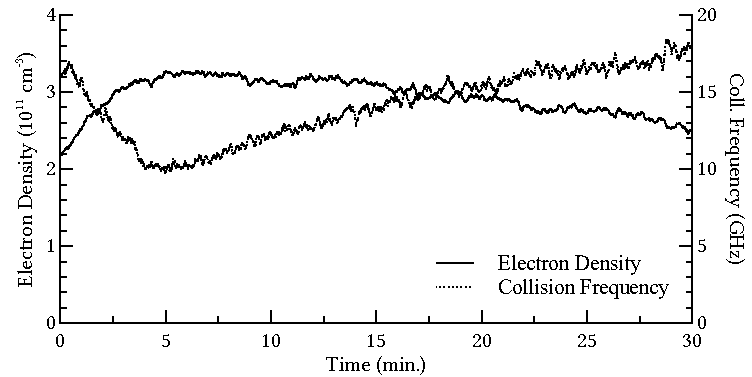
\includegraphics{./chapters/nasa/figures/densev.pdf}
  \caption{The evolution of the density (---) and the collision frequency
    (\raisebox{2.5pt}{${\scriptscriptstyle \centerdot \centerdot \centerdot}$}) in
    a \acs{rpnd} over a period of 30 minutes. These quantities reach their
    respective maximum and minimum after approximately five minutes, however these
    are not equilibrium values. The \acs{rpnd} continues to change over long
    durations.}
  \label{fig:densev}
\end{figure}
shows the calculation of the electron densities and collision frequencies from
the measured phase and amplitude changes. The data shown does not include the
operation of the DC sustainer. The data appear to confirm the concern that the
sealed vacuum chamber causes long-term variations in the plasma. The electron
density changes by nearly 50\% during the first five minutes of operation and is
followed by a slow decline over the next 25 minutes. Simultaneously, the
effective collisions frequency of the electrons ranges from 10-18 GHz. Overall,
the electron density ranged from 2.25-3.25 $\times10^{11}$ cm$^{-3}$. This is
somewhat less than the anticipated density. As previously noted, other studies
in \acs{fiw} discharges \cite{Aleksandrov2007, Pancheshnyi199, Macheret2006}
measured densities well in excess of 10$^{12}$ cm$^{-3}$.



$2.25\times 10^{11}$ cm$^{-3}$ to $3.25\times 10^{11}$ cm$^{-3}$. The magnitude
of the electron density is somewhat less than anticipated; other papers such as
\cite{Aleksandrov2007}, \cite{Pancheshnyi1999}, and \cite{Macheret2006} state
densities exceeding $10^{12}$ cm$^{-3}$. Separate experiments (not shown here)
demonstrated similar electron densities and collision frequencies. However, the
time for the system to reach its quasi-equilibrium varied and, in some cases,
required 10 minutes.

The observed increase in collision frequency was, perhaps, a result of
increasing pressure and gas temperature in the chamber. Meanwhile, the change in
electron density may be a result of a changing chemical composition. It is not
immediately clear what mechanism is responsible for this, but it is well-known
that electrons will readily attach to water molecules. As they are destroyed
through dissociation, the attachment rate would decline and it would be
reasonable to expect an increase in electron density.

\subsection{DC Sustainer}

Six separate experiments were run with the DC sustainer discharge on at
approximately 750 V (current limited), and four experiments were run with the
sustainer off (electrodes floating). Difficulties with \acs{emi} prevented a
more complete evaluation of the sustainer's effect. Therefore, an absolute
statement on the influence of the DC sustainer is not possible. However,
experiments without the DC sustainer exhibited consistently higher, but
variable, densities.

It is believed that the sustainer may have caused increased energy transfer to
the excited states of atoms and molecules, but was ineffective at increasing the
electron density. Indeed, the sustainer voltage was insufficient to produce a
glow discharge independent of the high voltage pulses. As such, one may conclude
that it will tend to extract more electrons than it produces. This being the
case, a DC sustainer may be useful in situations requiring fast gas heating, but
at the cost of a reduced ionization efficiency.

\section{Rotational Spectroscopy}

The approach used measured the rotational spectra of
a molecular system and used this information to infer the rotational
temperature. As a result of the close energy-spacing of the rotational levels,
this temperature is usually a good measure of the translational temperature of
the system \cite{Laux1993}. This technique is limited by the ability to detect
light from the transitions, and by the equilibration time of the translational
and rotational temperatures.

The measurement of rotational transitions is a common diagnostic for the
measurement of gas temperatures, particularly in the field of combustion.
Matching of the rotational spectra is typically accomplished with a computer
program such as Specair \cite{Laux2002} and LIFBASE \cite{Luque1999}. However, a
survey of the available programs revealed little documentation about the
calculation methods and none which provided the necessary flexibility how the
spectra were generated. This necessitated the development of a program to
automate the generation and matching of rotational spectra.
